%%%%%%%%%%%%%%%%%%%%%%%%%%%%%%%%%%%%%%%%%%%%%%%%%%%%%%%%%%%%%%%%%%%%%%%%
% Plantilla TFG/TFM
% Escuela Politécnica Superior de la Universidad de Alicante
% Realizado por: Jose Manuel Requena Plens
% Contacto: info@jmrplens.com / Telegram:@jmrplens
%%%%%%%%%%%%%%%%%%%%%%%%%%%%%%%%%%%%%%%%%%%%%%%%%%%%%%%%%%%%%%%%%%%%%%%%

\chapter{Estudio viabilidad}
\label{estudioviabilidad}
En este punto del proyecto se va a presentar una planificación temporal del proyecto, la planificación de los recursos y requisitos, además de una planificación de riesgos.
\section{Planificación temporal}
Para llegar a buen puerto en un proyecto es necesario intentar una buena estimación, que sabiendo que no es tarea fácil y difícil de cumplir, teniendo fechas de entrega continua al cliente podemos establecer prioridades y tomar decisiones estructurales en función de las necesidades temporales y de entrega. Como puede ser, por ejemplo, la entrada de nuevos requisitos que hacen retroceder otras funcionalidades en prioridad o que, incluso, las hacen quedar fuera del backlog; o que por problemas técnicos o por dificultad de implementación una tarea se retrase tanto que arrastre otras relacionadas.
\vspace{1em}
\par Cada hito realizado se asemeja bastante a las fases de la ingeniería de software y, a grandes rasgos, son los siguientes:
\begin{itemize}
    \item Hito 0 - Análisis:
    En este primer hito se realiza la primera ronda de contacto con los temas relacionados del proyecto. En este proyecto han sido el estudio de la disponibilidad web low-cost y acercarnos al banco de alimentos a ver en vivo el trabajo y necesidades de los voluntarios.
    \item Hito 1 - Especificación:
    En este hito se realizan los estudios y la documentación tanto del estado del arte como de las herramientas a utilizar. Además, se especifican los requisitos, los riesgos y se documentan los casos de uso y los diagramas.
    \item Hito 2 - Fase de desarrollo:
    Éste es el hito más largo y complicado, consiste en realizar el desarrollo del la apliacción backend, diseño e implementación de bases de datos y desarrollo del frontend.
    \item Hito 3 - Fase de pruebas:
    Último hito, en este se realizan pruebas de integración y satisfaccción además de revisar y finalizar la memoria.
\end{itemize}
\vspace{1em}
\par En este proyecto la planificación temporal empezó una vez llegados al hito 2, se ha usado la funcionalidad de Canvan, Issues y Milestone que proporciona Github en su plataforma.
\begin{figure}[h]
\centering
\begin{tabular}{ccc}
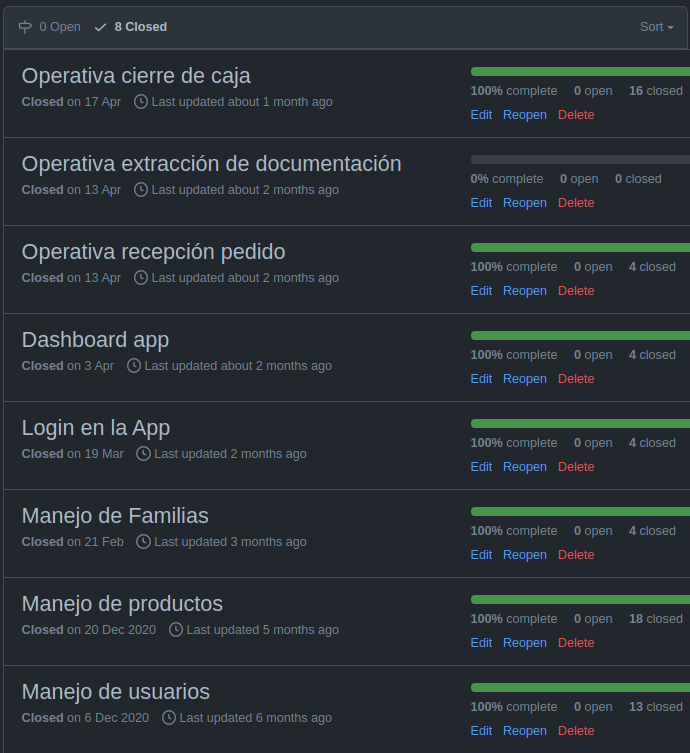
\includegraphics[scale=0.62]{archivos/github_milestones.png}
\end{tabular}
\caption{Milestones cerradas en Github}
\label{fig:github_milestones}
\end{figure}
\clearpage
\section{Gestión de riesgos}
Una de los aspectos más importantes de la planificación de un proyecto es una buena prevención de los riesgos y contratiempos que se puedan ocasionar durante la realización del proyecto. Tanto si deben ser mitigables sin falta o si se pueden asumir. Para ello se documentan y se establecen pautas que especifiquen cómo se resuelve cada riesgo, éstos se identifican de la siguiente manera:
\begin{itemize}
    \item Identificador: código de identificación
    \item Nombre: Palabra o conjunto de palabras breves y descriptivas
    \item Probabilidad: posibilidad de que ocurra dicho riesgo
    \item Consecuencia: nivel de importancia de que ocurra el riesgo
    \item Estrategia: pautas a seguir para resolver el riesgo
\end{itemize}

%%%%%%%%%%%%
%% Riesgo %%
%%%%%%%%%%%%
\vspace{1em}
\par
\begin{tabular}{||p{3cm}|p{11cm}||} 
\hline
Identificador & R1 \\ [0.5ex] 
\hline\hline
Nombre & No disponer de hosting \\ 
\hline
Tipo & Tecnología \\
\hline
Probabilidad & Media \\
\hline
Efectos & Serio \\
\hline
Estrategia & Obtener presupuestos \\ [1ex] 
\hline
\end{tabular}

%%%%%%%%%%%%
%% Riesgo %%
%%%%%%%%%%%%
\vspace{1em}
\par
\begin{tabular}{||p{3cm}|p{11cm}||} 
\hline
Identificador & R2 \\ [0.5ex] 
\hline\hline
Nombre & Caída del hosting \\ 
\hline
Tipo & Tecnología \\
\hline
Probabilidad & Baja \\
\hline
Efectos & Serio \\
\hline
Estrategia & Obtener presupuestos alta disponibilidad o esperar a su recuperación \\ [1ex] 
\hline
\end{tabular}

%%%%%%%%%%%%
%% Riesgo %%
%%%%%%%%%%%%
\vspace{1em}
\par
\begin{tabular}{||p{3cm}|p{11cm}||} 
\hline
Identificador & R3 \\ [0.5ex] 
\hline\hline
Nombre & Conocimientos innecesarios \\ 
\hline
Tipo & Persona \\
\hline
Probabilidad & Media \\
\hline
Efectos & Serio \\
\hline
Estrategia & Revisar documentación y vídeo tutoriales entregados \\ [1ex] 
\hline
\end{tabular}

%%%%%%%%%%%%
%% Riesgo %%
%%%%%%%%%%%%
\vspace{1em}
\par
\begin{tabular}{||p{3cm}|p{11cm}||} 
\hline
Identificador & R4 \\ [0.5ex] 
\hline\hline
Nombre & Acumulación de tareas \\ 
\hline
Tipo & Organizacional \\
\hline
Probabilidad & Media \\
\hline
Efectos & Serio \\
\hline
Estrategia & Buena planificación y gestión de tiempos \\ [1ex] 
\hline
\end{tabular}

%%%%%%%%%%%%
%% Riesgo %%
%%%%%%%%%%%%
\vspace{1em}
\par
\begin{tabular}{||p{3cm}|p{11cm}||} 
\hline
Identificador & R5 \\ [0.5ex] 
\hline\hline
Nombre & Licencias de herramientas \\ 
\hline
Tipo & Herramientas \\
\hline
Probabilidad & Media \\
\hline
Efectos & Tolerable \\
\hline
Estrategia & Asumir costes o adoptar herramientas libres \\ [1ex] 
\hline
\end{tabular}

%%%%%%%%%%%%
%% Riesgo %%
%%%%%%%%%%%%
\vspace{1em}
\par
\begin{tabular}{||p{3cm}|p{11cm}||} 
\hline
Identificador & R6 \\ [0.5ex] 
\hline\hline
Nombre & Bugs \\ 
\hline
Tipo & Herramientas \\
\hline
Probabilidad & Media \\
\hline
Efectos & Serio \\
\hline
Estrategia & Seguir metodología para arreglar y entregar rápido \\ [1ex] 
\hline
\end{tabular}

%%%%%%%%%%%%
%% Riesgo %%
%%%%%%%%%%%%
\vspace{1em}
\par
\begin{tabular}{||p{3cm}|p{11cm}||} 
\hline
Identificador & R7 \\ [0.5ex] 
\hline\hline
Nombre & Nueva funcionalidad \\ 
\hline
Tipo & Requerimientos \\
\hline
Probabilidad & Alta \\
\hline
Efectos & Serio \\
\hline
Estrategia & Seguir metodología para desarrollar y entregar rápido \\ [1ex] 
\hline
\end{tabular}

%%%%%%%%%%%%
%% Riesgo %%
%%%%%%%%%%%%
\vspace{1em}
\par
\begin{tabular}{||p{3cm}|p{11cm}||} 
\hline
Identificador & R8 \\ [0.5ex] 
\hline\hline
Nombre & Cambios en las bases de datos \\ 
\hline
Tipo & Requerimientos \\
\hline
Probabilidad & Alta \\
\hline
Efectos & Tolerable \\
\hline
Estrategia & Mongodb minimiza el impacto por su flexibilidad \\ [1ex] 
\hline
\end{tabular}

%%%%%%%%%%%%
%% Riesgo %%
%%%%%%%%%%%%
\vspace{1em}
\par
\begin{tabular}{||p{3cm}|p{11cm}||} 
\hline
Identificador & R9 \\ [0.5ex] 
\hline\hline
Nombre & Pérdida de trabajo \\ 
\hline
Tipo & Herramientas \\
\hline
Probabilidad & Baja \\
\hline
Efectos & Serio \\
\hline
Estrategia & Hacer copias de seguridad de forma recurrente \\ [1ex] 
\hline
\end{tabular}

%%%%%%%%%%%%
%% Riesgo %%
%%%%%%%%%%%%
\vspace{1em}
\par
\begin{tabular}{||p{3cm}|p{11cm}||} 
\hline
Identificador & R10 \\ [0.5ex] 
\hline\hline
Nombre & Modificaciones en el frontend \\ 
\hline
Tipo & Requerimientos \\
\hline
Probabilidad & Alta \\
\hline
Efectos & Tolerable \\
\hline
Estrategia & Seguir metodología para desarrollar y entregar rápido \\ [1ex] 
\hline
\end{tabular}

%%%%%%%%%%%%
%% Riesgo %%
%%%%%%%%%%%%
\vspace{1em}
\par
\begin{tabular}{||p{3cm}|p{11cm}||} 
\hline
Identificador & R11 \\ [0.5ex] 
\hline\hline
Nombre & Infraestimar tiempo de desarrollo \\ 
\hline
Tipo & Estimación \\
\hline
Probabilidad & Media \\
\hline
Efectos & Serio \\
\hline
Estrategia & Organizar tareas con margen suficiente \\ [1ex] 
\hline
\end{tabular}

%%%%%%%%%%%%
%% Riesgo %%
%%%%%%%%%%%%
\vspace{1em}
\par
\begin{tabular}{||p{3cm}|p{11cm}||} 
\hline
Identificador & R12 \\ [0.5ex] 
\hline\hline
Nombre & Falta de realización de alguna parte del proyecto \\ 
\hline
Tipo & Estimación \\
\hline
Probabilidad & Media \\
\hline
Efectos & Serio \\
\hline
Estrategia & Documentar funcionalidades pendientes y continuar desarrollo \\ [1ex] 
\hline
\end{tabular}

\chapter{Especificación de requisitos}
\label{requisitos}
En esta sección se van a detallar los objetivos del sistema para, a partir de ahí, obtener los casos de uso y así los requisitos del proyecto.
\section{Objetivos del sistema}
Para poder comenzar a establecer los requisitos se deben establecer los objetivos que tiene el sistema, para ello vamos a mostrarlo en formato de tabla en la que se detalla cada objetivo con su descripción y prioridad.

%%%%%%%%%%%%%%
%% Objetivo %%
%%%%%%%%%%%%%%
\vspace{1em}
\par
\begin{tabular}{||p{3cm}|p{11cm}||} 
\hline
Identificador & O1 \\ [0.5ex] 
\hline\hline
Nombre & Gestión de usuarios \\ 
\hline
Descripción & Se debe ser capaz de crear y loguear usuarios \\
\hline
Prioridad & Alta \\ [1ex] 
\hline
\end{tabular}

%%%%%%%%%%%%%%
%% Objetivo %%
%%%%%%%%%%%%%%
\vspace{1em}
\par
\begin{tabular}{||p{3cm}|p{11cm}||} 
\hline
Identificador & O2 \\ [0.5ex] 
\hline\hline
Nombre & Gestión de almacenes \\ 
\hline
Descripción & Se debe ser capaz de crear y editar almacenes \\
\hline
Prioridad & Alta \\ [1ex] 
\hline
\end{tabular}

%%%%%%%%%%%%%%
%% Objetivo %%
%%%%%%%%%%%%%%
\vspace{1em}
\par
\begin{tabular}{||p{3cm}|p{11cm}||} 
\hline
Identificador & O3 \\ [0.5ex] 
\hline\hline
Nombre & Gestión de productos \\ 
\hline
Descripción & Se debe ser capaz de crear y editar productos \\
\hline
Prioridad & Alta \\ [1ex] 
\hline
\end{tabular}

%%%%%%%%%%%%%%
%% Objetivo %%
%%%%%%%%%%%%%%
\vspace{1em}
\par
\begin{tabular}{||p{3cm}|p{11cm}||} 
\hline
Identificador & O4 \\ [0.5ex] 
\hline\hline
Nombre & Gestión de roles de usuario \\ 
\hline
Descripción & Se debe diferenciar permisos por roles de usuario \\
\hline
Prioridad & Alta \\ [1ex] 
\hline
\end{tabular}

%%%%%%%%%%%%%%
%% Objetivo %%
%%%%%%%%%%%%%%
\vspace{1em}
\par
\begin{tabular}{||p{3cm}|p{11cm}||} 
\hline
Identificador & O5 \\ [0.5ex] 
\hline\hline
Nombre & Gestión de familias \\ 
\hline
Descripción & Se deben recordar las familias por limitaciones en el mismo mes \\
\hline
Prioridad & Alta \\ [1ex] 
\hline
\end{tabular}

%%%%%%%%%%%%%%
%% Objetivo %%
%%%%%%%%%%%%%%
\vspace{1em}
\par
\begin{tabular}{||p{3cm}|p{11cm}||} 
\hline
Identificador & O6 \\ [0.5ex] 
\hline\hline
Nombre & Recepción de pedidos de compra \\ 
\hline
Descripción & Se debe gestionar el proceso de compra con la memoria por familia \\
\hline
Prioridad & Alta \\ [1ex] 
\hline
\end{tabular}


%%%%%%%%%%%%%%
%% Objetivo %%
%%%%%%%%%%%%%%
\vspace{1em}
\par
\begin{tabular}{||p{3cm}|p{11cm}||} 
\hline
Identificador & O7 \\ [0.5ex] 
\hline\hline
Nombre & Gestión de cobros y caja \\ 
\hline
Descripción & Se deben poder marcar pedidos como cobrados o erróneos \\
\hline
Prioridad & Alta \\ [1ex] 
\hline
\end{tabular}


%%%%%%%%%%%%%%
%% Objetivo %%
%%%%%%%%%%%%%%
\vspace{1em}
\par
\begin{tabular}{||p{3cm}|p{11cm}||} 
\hline
Identificador & O8 \\ [0.5ex] 
\hline\hline
Nombre & Gestión de expedición de pedidos \\ 
\hline
Descripción & Se deben poder ver pedidos a entregar y marcarlos entregados \\
\hline
Prioridad & Alta \\ [1ex] 
\hline
\end{tabular}


%%%%%%%%%%%%%%
%% Objetivo %%
%%%%%%%%%%%%%%
\vspace{1em}
\par
\begin{tabular}{||p{3cm}|p{11cm}||} 
\hline
Identificador & O9 \\ [0.5ex] 
\hline\hline
Nombre & Dashboard con estadísticas \\ 
\hline
Descripción & Se debe añadir información relevante de forma resumida y legible \\
\hline
Prioridad & Media \\ [1ex] 
\hline
\end{tabular}


%%%%%%%%%%%%%%
%% Objetivo %%
%%%%%%%%%%%%%%
\vspace{1em}
\par
\begin{tabular}{||p{3cm}|p{11cm}||} 
\hline
Identificador & O10 \\ [0.5ex] 
\hline\hline
Nombre & Imprimir facturas \\ 
\hline
Descripción & Se deben mostrar las facturas maquetadas para imprimirlas \\
\hline
Prioridad & Alta \\ [1ex] 
\hline
\end{tabular}


%%%%%%%%%%%%%%
%% Objetivo %%
%%%%%%%%%%%%%%
\vspace{1em}
\par
\begin{tabular}{||p{3cm}|p{11cm}||} 
\hline
Identificador & O11 \\ [0.5ex] 
\hline\hline
Nombre & Anonimización de facturas \\ 
\hline
Descripción & Se debe poder desvincular facturas de las familias \\
\hline
Prioridad & Media \\ [1ex] 
\hline
\end{tabular}


%%%%%%%%%%%%%%
%% Objetivo %%
%%%%%%%%%%%%%%
\vspace{1em}
\par
\begin{tabular}{||p{3cm}|p{11cm}||} 
\hline
Identificador & O12 \\ [0.5ex] 
\hline\hline
Nombre & Productos con información nutricional \\ 
\hline
Descripción & Se debe tener información automatizada de los productos \\
\hline
Prioridad & Baja \\ [1ex] 
\hline
\end{tabular}

%%%%%%%%%%%%%%
%% Objetivo %%
%%%%%%%%%%%%%%
\vspace{1em}
\par
\begin{tabular}{||p{3cm}|p{11cm}||} 
\hline
Identificador & O13 \\ [0.5ex] 
\hline\hline
Nombre & Leer EAN de los productos \\ 
\hline
Descripción & Se debe poder vincular EAN al producto mediante cámara o lector \\
\hline
Prioridad & Baja \\ [1ex] 
\hline
\end{tabular}

\section{Casos de uso}
Los casos de uso sirven para ilustrar el comportamiento del sistema con un agente externo. Permite ver el alcance y límites del sistema y su relación con el entorno. Para poder realizar los casos de uso se deben identificar los agentes externos.
\vspace{1em}
\par En este sistema hay varios agentes, éstos son:
\begin{itemize}
    \item Usuario con uno o más roles:
    \begin{itemize}
        \item Recepción pedidos
        \begin{itemize}
            \item Búsqueda de familias
            \item Recepción de pedidos y visualización de facturas
        \end{itemize}
        \item Caja
        \begin{itemize}
            \item Gestión de caja y facturas
        \end{itemize}
        \item Almacén
        \begin{itemize}
            \item Expedición de pedidos
            \item Gestión de productos, añadir, editar y borrar
        \end{itemize}
        \item Administrador
        \begin{itemize}
            \item Todo lo anterior
            \item Añadir usuarios y editarlos
            \item Activar y desactivar usuarios
            \item Dar o quitar roles
            \item Anonimizar facturas
        \end{itemize}
    \end{itemize}
    \item Usuario súper administrador
    \begin{itemize}
        \item Igual que administrador pero no puede perder su rol
        \item Se deben crear a mano por un desarrollador con acceso al sistema
    \end{itemize}
\end{itemize}
\clearpage
Ahora se van a clasificar cada caso de uso de una forma similar a los objetivos, con los siguientes datos: identificador, nombre, descripción, flujo básico, flujos alternos, pre-condiciones, post-condiciones.

%%%%%%%%%%%%%%%%%
%% Caso de uso %%
%%%%%%%%%%%%%%%%%
\vspace{1em}
\par
\begin{tabular}{||p{3cm}|p{11cm}||} 
\hline
Identificador & CU1 \\ [0.5ex] 
\hline\hline
Nombre & Iniciar \\ 
\hline
Descripción & Iniciar sesión \\
\hline
Pre-condiciones & Debe estar registrado \\
\hline
Flujo básico & Carga la página principal, escribe sus datos en el formulario
y envía el formulario \\
\hline
Flujo alterno & - \\
\hline
Post-condiciones &
\begin{itemize}
    \item Login correcto: Se muestra el dashboard
    \item Login incorrecto: Se muestra mensaje de datos incorrectos
\end{itemize} \\
\hline
\end{tabular}

%%%%%%%%%%%%%%%%%
%% Caso de uso %%
%%%%%%%%%%%%%%%%%
\vspace{1em}
\par
\begin{tabular}{||p{3cm}|p{11cm}||} 
\hline
Identificador & CU2 \\ [0.5ex] 
\hline\hline
Nombre & Crear usuario \\ 
\hline
Descripción & Permite al administrador crear un usuario nuevo \\
\hline
Pre-condiciones & Debe tener rol Administrador \\
\hline
Flujo básico & Login correcto y navega a creación de usuarios. Introduce los datos nuevos y pulsa crear. \\
\hline
Flujo alterno & - \\
\hline
Post-condiciones &
\begin{itemize}
    \item Crear correcto: Se muestra mensaje verde de confirmación
    \item Crear incorrecto: Se muestra mensaje rojo con información del error
\end{itemize} \\
\hline
\end{tabular}

%%%%%%%%%%%%%%%%%
%% Caso de uso %%
%%%%%%%%%%%%%%%%%
\vspace{1em}
\par
\begin{tabular}{||p{3cm}|p{11cm}||} 
\hline
Identificador & CU3 \\ [0.5ex] 
\hline\hline
Nombre & Editar usuario \\ 
\hline
Descripción & Permite al administrador cambiar los datos del usuario \\
\hline
Pre-condiciones & Debe tener rol Administrador \\
\hline
Flujo básico & Login correcto y navega al detalle de un usuario. Cambia los datos y pulsa guardar. \\
\hline
Flujo alterno & - \\
\hline
Post-condiciones &
\begin{itemize}
    \item Edición correcto: Se muestra mensaje verde de confirmación
    \item Edición incorrecto: Se muestra mensaje rojo con información del error
\end{itemize} \\
\hline
\end{tabular}

%%%%%%%%%%%%%%%%%
%% Caso de uso %%
%%%%%%%%%%%%%%%%%
\vspace{1em}
\par
\begin{tabular}{||p{3cm}|p{11cm}||} 
\hline
Identificador & CU4 \\ [0.5ex] 
\hline\hline
Nombre & Buscar familia \\ 
\hline
Descripción & Permite al usuario buscar familia por identificación o por expediente \\
\hline
Pre-condiciones & Debe tener rol Pedidos \\
\hline
Flujo básico & Login correcto y navega a pedidos y usa el formulario de búsqueda de familias \\
\hline
Flujo alterno & - \\
\hline
Post-condiciones &
\begin{itemize}
    \item Búsqueda con coincidencias: Se muestra en la página de pedidos información sobre la familia ese mes
    \item Búsqueda sin coincidencias: En la página de pedidos no aparece información sobre la familia ese mes
\end{itemize} \\
\hline
\end{tabular}

%%%%%%%%%%%%%%%%%
%% Caso de uso %%
%%%%%%%%%%%%%%%%%
\vspace{1em}
\par
\begin{tabular}{||p{3cm}|p{11cm}||} 
\hline
Identificador & CU5 \\ [0.5ex] 
\hline\hline
Nombre & Crear pedido \\ 
\hline
Descripción & Permite al usuario crear un pedido nuevo teniendo en cuenta limitaciones del expediente \\
\hline
Pre-condiciones & Debe tener rol Pedidos \\
\hline
Flujo básico & Login correcto y navega a pedidos, usa el formulario de búsqueda de familias y comienza el proceso de pedido hasta la generación de la factura \\
\hline
Flujo alterno & - \\
\hline
Post-condiciones & - \\
\hline
\end{tabular}

%%%%%%%%%%%%%%%%%
%% Caso de uso %%
%%%%%%%%%%%%%%%%%
\vspace{1em}
\par
\begin{tabular}{||p{3cm}|p{11cm}||} 
\hline
Identificador & CU6 \\ [0.5ex] 
\hline\hline
Nombre & Imprimir factura \\ 
\hline
Descripción & Permite al usuario ver la factura maquetada para impresión \\
\hline
Pre-condiciones & Debe estar registrado \\
\hline
Flujo básico & Login correcto y en la tabla de facturas del día, click en el ojo de la que quiera ver \\
\hline
Flujo alterno & Flujo de pedido y al dar click a generar factura se abre una pestaña nueva con ésta lista para imprimir \\
\hline
Post-condiciones & - \\
\hline
\end{tabular}

%%%%%%%%%%%%%%%%%
%% Caso de uso %%
%%%%%%%%%%%%%%%%%
\vspace{1em}
\par
\begin{tabular}{||p{3cm}|p{11cm}||} 
\hline
Identificador & CU7 \\ [0.5ex] 
\hline\hline
Nombre & Crear almacén \\ 
\hline
Descripción & Permite al usuario crear un almacén nuevo para separar stocks, facturas y expedición \\
\hline
Pre-condiciones & Debe tener rol Administrador \\
\hline
Flujo básico & Login correcto y navega a gestión de almacenes, pulsa crear y completa el formulario de creación \\
\hline
Flujo alterno & - \\
\hline
Post-condiciones &
\begin{itemize}
    \item Crear correcto: Se muestra mensaje verde de confirmación
    \item Crear incorrecto: Se muestra mensaje rojo con información del error
\end{itemize} \\
\hline
\end{tabular}

%%%%%%%%%%%%%%%%%
%% Caso de uso %%
%%%%%%%%%%%%%%%%%
\vspace{1em}
\par
\begin{tabular}{||p{3cm}|p{11cm}||} 
\hline
Identificador & CU8 \\ [0.5ex] 
\hline\hline
Nombre & Editar almacén \\ 
\hline
Descripción & Permite al usuario cambiar los datos del almacén \\
\hline
Pre-condiciones & Debe tener rol Administrador \\
\hline
Flujo básico & Login correcto y navega a gestión de almacenes, pulsa editar el almacén de la lista y edita los datos en el formulario \\
\hline
Flujo alterno & - \\
\hline
Post-condiciones &
\begin{itemize}
    \item Editar correcto: Se muestra mensaje verde de confirmación
    \item Editar incorrecto: Se muestra mensaje rojo con información del error
\end{itemize} \\
\hline
\end{tabular}

%%%%%%%%%%%%%%%%%
%% Caso de uso %%
%%%%%%%%%%%%%%%%%
\vspace{1em}
\par
\begin{tabular}{||p{3cm}|p{11cm}||} 
\hline
Identificador & CU9 \\ [0.5ex] 
\hline\hline
Nombre & Crear producto \\ 
\hline
Descripción & Permite al usuario crear un producto \\
\hline
Pre-condiciones & Debe tener rol Almacén \\
\hline
Flujo básico & Login correcto y navega a gestión de productos, pulsa crear y completa el formulario de creación \\
\hline
Flujo alterno & Login correcto y navega a gestión de productos, pulsa crear y completa el formulario de creación, además usa la webcam para leer el código EAN y se recupera la información nutricional pidiéndola a OpenFoodFacts \\
\hline
Post-condiciones &
\begin{itemize}
    \item Crear correcto: Se muestra mensaje verde de confirmación
    \item Crear incorrecto: Se muestra mensaje rojo con información del error
\end{itemize} \\
\hline
\end{tabular}

%%%%%%%%%%%%%%%%%
%% Caso de uso %%
%%%%%%%%%%%%%%%%%
\vspace{1em}
\par
\begin{tabular}{||p{3cm}|p{11cm}||} 
\hline
Identificador & CU10 \\ [0.5ex] 
\hline\hline
Nombre & Editar producto \\ 
\hline
Descripción & Permite al usuario editar un producto \\
\hline
Pre-condiciones & Debe tener rol Almacén \\
\hline
Flujo básico & Login correcto y navega a gestión de productos, pulsa editar en el producto que quiera de la lista y edita los datos en el formulario \\
\hline
Flujo alterno & - \\
\hline
Post-condiciones &
\begin{itemize}
    \item Editar correcto: Se muestra mensaje verde de confirmación
    \item Editar incorrecto: Se muestra mensaje rojo con información del error
\end{itemize} \\
\hline
\end{tabular}

%%%%%%%%%%%%%%%%%
%% Caso de uso %%
%%%%%%%%%%%%%%%%%
\vspace{1em}
\par
\begin{tabular}{||p{3cm}|p{11cm}||} 
\hline
Identificador & CU11 \\ [0.5ex] 
\hline\hline
Nombre & Cobrar un pedido \\ 
\hline
Descripción & Permite al usuario marcar un pedido pendiente como cobrado \\
\hline
Pre-condiciones & Debe tener rol Caja \\
\hline
Flujo básico & Login correcto y navega a caja, pulsa en cobrar la factura que considere \\
\hline
Flujo alterno & - \\
\hline
Post-condiciones & - \\
\hline
\end{tabular}

%%%%%%%%%%%%%%%%%
%% Caso de uso %%
%%%%%%%%%%%%%%%%%
\vspace{1em}
\par
\begin{tabular}{||p{3cm}|p{11cm}||} 
\hline
Identificador & CU12 \\ [0.5ex] 
\hline\hline
Nombre & Rechazar un pedido \\ 
\hline
Descripción & Permite al usuario marcar un pedido pendiente como anulado \\
\hline
Pre-condiciones & Debe tener rol Caja \\
\hline
Flujo básico & Login correcto y navega a caja, pulsa en anular la factura que considere \\
\hline
Flujo alterno & - \\
\hline
Post-condiciones & - \\
\hline
\end{tabular}

%%%%%%%%%%%%%%%%%
%% Caso de uso %%
%%%%%%%%%%%%%%%%%
\vspace{1em}
\par
\begin{tabular}{||p{3cm}|p{11cm}||} 
\hline
Identificador & CU13 \\ [0.5ex] 
\hline\hline
Nombre & Expedir un pedido \\ 
\hline
Descripción & Permite al usuario marcar un pedido sin expedir como expedido \\
\hline
Pre-condiciones & Debe tener rol Almacén \\
\hline
Flujo básico & Login correcto y navega a almacén, pulsa en el pedido que considere, marca los productos conforme los va preparando y lo marca como expedido \\
\hline
Flujo alterno & - \\
\hline
Post-condiciones & - \\
\hline
\end{tabular}

%%%%%%%%%%%%%%%%%
%% Caso de uso %%
%%%%%%%%%%%%%%%%%
\vspace{1em}
\par
\begin{tabular}{||p{3cm}|p{11cm}||} 
\hline
Identificador & CU14 \\ [0.5ex] 
\hline\hline
Nombre & Anonimizar facturas \\ 
\hline
Descripción & Permite al usuario, por rango de fechas, anonimizar facturas para desvincular datos de compra a datos personales \\
\hline
Pre-condiciones & Debe tener rol Administrador \\
\hline
Flujo básico & Login correcto y navega a caja, busca facturas en el rango que considere y pulsa el botón anonimizar facturas \\
\hline
Flujo alterno & - \\
\hline
Post-condiciones & - \\
\hline
\end{tabular}
